\section{Motivação e Conceitos Básicos}
\subsection{Caso Motivador}
Para exemplificar melhor o conceito de conflito de integração semântico, considere o cenário de exemplo da \hyperref[fig:codigo-motivador]{Figura 1}.\footnote{Assumindo um cenário de \emph{merge} formado por \emph{commits Base, Left, Right e Merge}, esse último contendo o arquivo apresentado na figura.} Conseguimos observar a classe \texttt{Text}, que contém três atributos: uma \emph{string}, que referencia o texto representado pelos objetos dessa classe e dois atributos do tipo inteiro, que correspondem à quantidade de correções aplicadas ao texto (remoção de espaços e palavras duplicadas), e a quantidade de comentários no texto. A classe \texttt{Text} também conta com o método \texttt{generateReport()} responsável por gerar o relatório da quantidade de \texttt{fixes} necessárias e comentários existentes.

Na \hyperref[fig:codigo-motivador]{Figura 1} é exibido o arquivo resultado da integração das mudanças em amarelo (Linha 6 foi adicionada pela versão \emph{Left}) e as mudanças em verde (Linha 8 foi adicionada pela versão \emph{Right}). As outras linhas de código são de uma versão \emph{Base}, o ancestral comum mais recente de ambas versões \emph{Left} e \emph{Right}\footnote{Para simplificar, assumimos um único ancestral comum (mais recente). As situações de \emph{Merge} cruzado no git, pode haver mais de um}. Nesse caso, podemos observar que as mudanças adicionadas por \emph{Left} e \emph{Right} não estão na mesma linha e nem em linhas consecutivas, assim as alterações podem ser \emph{textualmente} integradas com segurança e nenhum conflito seria reportado pelas ferramentas de \emph{Merge} atuais. 

\begin{figure}[!h]
    \begin{lstlisting}[escapechar=!]
    class Text {
        public String text;
        public int fixes;
        public int comments;
        void generateReport() {
+           !\colorbox{yellow}{countDuplicatedWhitespaces();}!
            countComments();
+           !\colorbox{green}{countDuplicatedWords();}!
        }
    }
    \end{lstlisting}
    \caption{Caso de exemplo de conflito integração semântico}
    \label{fig:codigo-motivador}
\end{figure}

Observando um pouco melhor as alterações de cada um dos desenvolvedores, assuma que \emph{Left}, ao adicionar a chamada do método \texttt{countDuplicatedWhitespaces()}, pretende realizar a contagem dos espaços em branco em um determinado texto e, ao final, sobrescreve o atributo \texttt{fixes} com o valor da contagem. Já \emph{Right}, adicionou a chamada ao método \texttt{countDuplicatedWords()} que sobrescreve \texttt{fixes} com o valor da contagem das palavras duplicadas no determinado texto. Entre as alterações de \emph{Left} e \emph{Right} temos um comando que vem de \emph{Base}. A chamada ao método \texttt{countComments()} realiza a contagem dos comentários no atributo \texttt{text}, mas diferente das demais chamadas de métodos, altera o atributo \texttt{comments}.

Apesar de a integração ter gerado um código sintaticamente válido e livre de conflitos textuais, a mudança feita por \emph{Right} interfere com a mudança feita por \emph{Left}, já que a execução da chamada ao \texttt{countDuplicateWords()} altera o valor do atributo \texttt{fixes}, que também é alterado pela chamada ao \texttt{countDuplicateWhitespace()}. Considerando que a intenção ou especificação da tarefa de \emph{Left} era exatamente armazenar em \texttt{fixes} a quantidade de espaços duplos, e que isso não acontece ao final da execução de \texttt{generateReport()}, quando \texttt{fixes} estará armazenando o número de palavras duplicadas, teremos então, um conflito semântico.\footnote{Mesmo que a implementação fosse outra, os resultados (de OA, conflito, interferência) poderiam ser os mesmos, assumindo especificações óbvias para o caso e o não conhecimento mútuo das tarefas de \emph{Left} e \emph{Right}} 

Em particular, a mudança feita por \emph{Right} inadvertidamente anula a mudança feita por \emph{Left}.
Para entender melhor porque há interferência nesse caso, considere o caso de teste ilustrado na \hyperref[fig:teste-motivador]{Figura 2}, escrito por \emph{Left} para confirmar que sua tarefa foi corretamente implementada.

\begin{figure}[h]
    \begin{lstlisting}[]
    public void countFixesTest() throws Throwable {
        Text t = new Text();
        t.text = "the the     dog dog";
        t.generateReport();
        assertTrue(1, t.fixes);
    }
    \end{lstlisting}
    \caption{Caso de teste que demonstra o conflito semântico na Figura 2.1}
    \label{fig:teste-motivador}
\end{figure}

O caso de teste executa o método \texttt{t.generateReport()}, utilizando como \emph{String} de entrada \texttt{‘‘the the\quad dog dog’’}. Se executarmos esse teste apenas na versão de \emph{Left} (sem a linha 8 Verde), o teste passará, pois existe apenas um espaço em branco no texto (entre as palavras \texttt{the} e \texttt{dog}). Já executando apenas no ramo de \emph{Right} (sem a linha 6 amarela) o teste falhará, pois \texttt{‘‘the the’’} e \texttt{‘‘dog dog’’} somam duas palavras duplicadas. Agora pensando apenas no cenário de \emph{merge} (\hyperref[fig:codigo-motivador]{Figura 1}) o teste também irá falhar, pois o último método a ser chamado é o \texttt{countDuplicatedWords()} adicionado por \emph{Right}, que sobrescreve \texttt{fixes} com o valor da quantidade de palavras duplicadas no texto.

Em isolado, ambos desenvolvedores implementaram suas tarefas corretamente, cumprindo os contratos que pretendiam. No entanto, devido a um detalhe da implementação adicionada pela versão \emph{Right}, o código integrado não cumpre o contrato pretendido pelo desenvolvedor de \emph{Left} (\texttt{fixes} deveria ser igual a 1). Perceba que a intenção de um dos desenvolvedores (\emph{Left}) não é preservada no \emph{merge}, ocorrendo assim uma interferência. 

Casos como esse, são muitas vezes difíceis e caros de se detectar e resolver. Na verdade, exceto em projetos que adotem boas práticas de escrita de código, práticas de revisão e tenha conjuntos de testes fortes, espera-se que a maioria dos conflitos semânticos escapem para os usuários. Mesmo com tais práticas, conflitos semânticos ainda são esperados. Se a detecção não for imediata após integração, pode ser ainda mais difícil corrigi-los, pois a resolução envolve a reconciliação da incompatibilidade semântica comportamental \cite{LeusonSilva2020}. Em nosso exemplo, teríamos que investigar se o defeito está nas implementações individuais de \emph{Left} e \emph{Right} ou em como um deles interfere no outro. Isto exigiria uma investigação não superficial que quebrasse os limites da abstração estabelecidos pelas declarações dos métodos chamados em \texttt{generateReport()}.

Para evitar esses problemas mencionados, bastaria executar a análise de substituição de atribuição proposta. No caso específico, nossa implementação detecta essa interferência, pois a análise de OA busca por alterações feitas por desenvolvedores diferentes, e que durante a execução, escrevem no mesmo componente do estado (\texttt{fixes}), sem atribuições intermediárias. De fato, a atribuição feita por \texttt{countDuplicateWhitespace()} em \texttt{fixes} é sobrescrita pela atribuição feita por \texttt{countDuplicatedWords()} e \texttt{countComments()} escreve em \texttt{comments}, não interferindo em \texttt{fixes}. 


\begin{figure}[!h]
    \begin{lstlisting}[escapechar=!]
right no método Text.countDuplicatedWords na linha 8, atribui o valor 2 a variável fixes e interfere em left no método Text.countDuplicatedWhitespaces na linha 6 que atribuiu o valor 1 para variável fixes.
    \end{lstlisting}
    \caption{Exemplo simplificado de um alerta reportado pela análise proposta}
    \label{fig:report-caso-motivador}
\end{figure}

Na \hyperref[fig:report-caso-motivador]{Figura 3}, temos um exemplo simplificado de um alerta reportado pela análise proposta.\footnote{Este é um exemplo simplificado para fins didáticos. A saída da ferramente pode ser um pouco diferente.} Os detalhes contêm a classe, o método, o número da linha e a instrução em que a substituição de atribuição aconteceu.

\subsection{Conceitos Básicos}

A definição de interferência localmente observável é inspirada na definição dada por Horwitz et al. \cite{Horwitz1989IntegratingNV}, que definiu um conflito de integração semântico como um cenário em que as contribuições das versões interferem entre si. Para ajudar a compreender melhor as definições que utilizamos neste trabalho, podemos observar a imagem ilustrada na  \hyperref[fig:analysis]{Figura 4}. Implementamos duas abordagens para detecção de OA em cenários de integração de código. OA \emph{intraprocedural} e OA \emph{interprocedural} são implementações que tentam ao máximo, dentro de suas características, uma aproximação para a definição da análise de substituição de atribuição OA. No que lhe concerne, OA é um tipo de interferência que busca identificar atribuições de dois desenvolvedores na mesma variável e atributos. Neste trabalho, utilizamos as interferências localmente observáveis, pois é a categoria de interferência que facilita a avaliação manual. Por fim, temos o conceito de interferência como aproximação para conflito, pois um conflito nada mais é do que interferência não intencional entre mudanças integradas dos desenvolvedores.

\begin{figure}[!h]
    \centering
    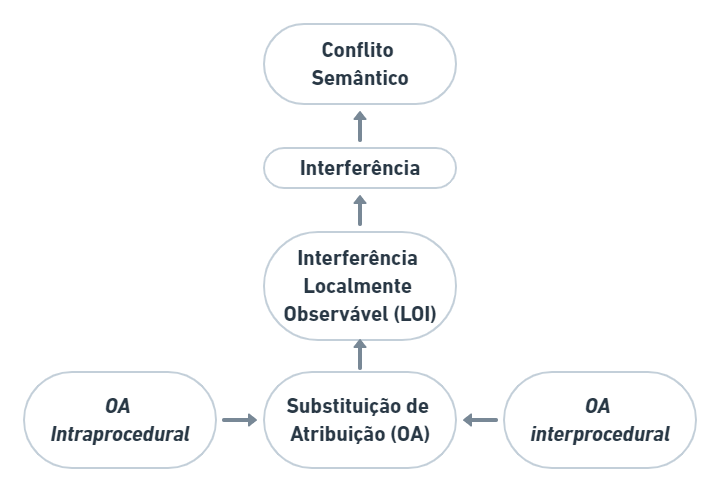
\includegraphics[width=0.8\linewidth]{images/analysis.png}
    \caption{Representação da hierarquia da análise até o conflito semântico}
    \label{fig:analysis}
\end{figure}

É importante ressaltar que OA e LOI são independentes, ou seja, para que um exista não é necessária a existência do outro.

Um exemplo de caso em que existe OA, mas não existe LOI, pode ser observado na imagem da \hyperref[fig:f3d6309]{Figura 5}. Não há LOI, pois \emph{Right} fez uma refatoração (\emph{extract variable} na variável \texttt{json}). No entanto, existe OA, pois os dois desenvolvedores atribuem a variável \texttt{setings}.

\begin{figure}[!h]
    \begin{lstlisting}[escapechar=!]
    public void testQueryModeCommonGramsAnalysis() {
       !\colorbox{yellow}{String json = "/org/elasticsearch/..."}!
        Settings settings = Settings.settingsBuilder()
            .loadFrom!\colorbox{yellow}{Stream(json, ...)}!
            .put("path.home", create!\colorbox{green}{Home}!())
            .build();
        }
    \end{lstlisting}
    \caption{Adaptação do Arquivo de \emph{merge} do cenário f3d6309 como exemplo de OA sem LOI}
    \label{fig:f3d6309}
\end{figure}

Para os casos em que não existe OA, mas existe LOI, temos o exemplo ilustrado na \hyperref[fig:3d4f995]{Figura 6}. Existe LOI, pois \emph{Right} está usando uma variável (\texttt{oplogDb}) alterada por \emph{Left}. Não existe OA, pois os desenvolvedores não sobrescrevem a mesma variável em nenhum momento.

\begin{figure}[!h]
    \begin{lstlisting}[escapechar=!]
    ...
    !\colorbox{yellow}{oplogDb = oplogDb.getMongo().getDB(...);}!
    ...
    !\colorbox{green}{oplogRefsCollection = oplogDb.getCollection(...);}!
    ...
    \end{lstlisting}
     \caption{Adaptação do arquivo de \emph{merge} do cenário 3d4f995 como exemplo de LOI sem OA}
    \label{fig:3d4f995}
\end{figure}